\documentclass[11pt]{article}
\usepackage[paperwidth=254mm,paperheight=142.875mm,margin=12mm]{geometry}
\usepackage{amsmath,amssymb}
\usepackage{graphicx}\graphicspath{{../}}

\newcommand{\R}{\mathbb{R}}

\begin{document}

\begin{center}
{\LARGE\bfseries Background notes}\par\vspace{4pt}
{\large Supporting material for understanding the paper. Not presented.}
\end{center}
\vspace{6pt}\hrule\vspace{10pt}

\paragraph{Quantization in one example (illustrative numbers).} Weights $x=(0.9,\,-0.3,\,0.1,\,0.6)$, $k=2$ bits, integers $\{0,1,2,3\}$.
\begin{enumerate}
\item Grid: smallest value $\to 0$, largest $\to 3$: $s_f=\dfrac{0.9-(-0.3)}{3}=0.4$, $b_f=-0.3$.
\item Rescale: $f(x)=(x+0.3)/0.4=(3,\,0,\,1,\,2.25)$.
\item Round: $q=(3,\,0,\,1,\,2)$. Stored: 2 bits per weight, plus $s_f$, $b_f$.
\item Back: $\hat x=0.4\,q-0.3=(0.9,\,-0.3,\,0.1,\,0.5)$. The last weight moved $0.6\to0.5$: the rounding error $s_f\delta$.
\end{enumerate}
Ridge instead maps $q$ back to $(0.935,\,-0.285,\,0.122,\,0.528)$: the error is spread over all four weights, total squared error $0.010\to0.007$.

\clearpage
\section{Chain rule}

\paragraph{Setup.} Let $h:\R^n\to\R^m$ be one layer and $\ell:\R^m\to\R$ be everything after it (the rest of the network and the loss), so the loss is $L(x)=\ell\big(h(x)\big)$. The \emph{local Jacobian} of the layer is the $m\times n$ matrix
\[
J_h(x)=\frac{\partial h}{\partial x},\qquad (J_h)_{ij}=\frac{\partial h_i}{\partial x_j}.
\]

\paragraph{Chain rule.}
\[
\nabla_x L \;=\; J_h(x)^{\top}\,\nabla \ell\big(h(x)\big).
\]
Here $\nabla \ell\big(h(x)\big)$ is the \emph{downstream gradient} (what the rest of the network wants the layer's output to do), and $J_h(x)^{\top}$ converts it into a gradient on the layer's input $x$.

\paragraph{Intuition.} The downstream gradient says how the loss would change if the layer's \emph{output} moved. The local Jacobian says how the layer's output moves when its \emph{input} $x$ moves. Multiplying the two gives how the loss changes when $x$ moves, which is what gradient descent needs to update $x$. Backpropagation repeats this layer by layer, so every layer's local Jacobian is a factor in the gradient that reaches earlier layers.

\paragraph{Two cases relevant to this paper.}
\begin{enumerate}
\item \textbf{Local Jacobian is zero}, $J_h(x)=0$. Then
\[
\nabla_x L = 0 \quad\text{for every downstream gradient}.
\]
\emph{Meaning:} small changes to $x$ do not change the layer's output, so the loss gives $x$ no direction to move. Gradient descent never updates $x$, and nothing before this layer learns either. This is what rounding (quantization) does.

\item \textbf{Local Jacobian is the identity}, $J_h(x)=I$. Then
\[
\nabla_x L = \nabla \ell\big(h(x)\big).
\]
\emph{Meaning:} the downstream gradient is passed back unchanged, as if the layer did nothing. Whatever the layer actually did to $x$ (for example, adding a rounding error) has no effect on the gradient, so earlier layers get no signal about it. This is what the Straight-Through Estimator (STE) assumes.
\end{enumerate}

\section{Ridge regression}

\paragraph{Why needed.} The paper's dequantizer $g$ is a ridge-regression fit of the original $x$ from the rounded $q$ (with $u=q$, $v=x$ below).

\paragraph{Notation.} For $u,v\in\R^N$: $\bar u=\frac1N\sum_i u_i$, $\overline{uv}=\frac1N\sum_i u_iv_i$, $\operatorname{Var}_u=\overline{u^2}-\bar u^{2}$, $\operatorname{Cov}_{uv}=\overline{uv}-\bar u\,\bar v$, and $\mathbf 1$ is the all-ones vector.

\paragraph{Problem.} Fit $v\approx a\,u+c\mathbf 1$, penalizing only the slope:
\[
\min_{a,c}\ \frac{1}{2N}\|a\,u+c\mathbf 1-v\|^2+\frac{\lambda}{2}a^2,\qquad \lambda>0 .
\]
Setting derivatives to zero:
\[
c^*=\bar v-a^*\bar u,\qquad a^*=\frac{\operatorname{Cov}_{uv}}{\operatorname{Var}_u+\lambda}.
\]
Without intercept ($c=0$): $a^*=\dfrac{\overline{uv}}{\overline{u^2}+\lambda}$.

\paragraph{Fit.} The vector of the line's predictions at the data points:
\[
\text{fit}=a^*u+c^*\mathbf 1=a^*(u-\bar u\mathbf 1)+\bar v\mathbf 1 .
\]

\paragraph{Role of $\lambda$.} (i) \emph{Stability:} the denominator is at least $\lambda>0$, so no division by zero even if all $u_i$ are equal. (ii) \emph{Shrinkage:} as $\lambda\to\infty$, $a^*\to0$ and the fit becomes the mean $\bar v\mathbf 1$.

\section{Quantization}

\paragraph{In short.} We select a grid of integers, assign one integer to each of our real numbers (rescale, then round to the nearest), and then try to get our real numbers back from those integers. Only the integers (plus one $s_f$, $b_f$ per block) are stored; the recovery is approximate, and the gap is the rounding error. The paper keeps the first two steps and changes only the last one: how to get back from the integers to the best possible real numbers.

\paragraph{Setup.} A block $x\in\R^N$ (weights or activations) is mapped to a $k$-bit integer grid $\{q_{\min},\dots,q_{\max}\}$ with $2^k$ levels. Notation A$a$W$w$: $a$-bit activations, $w$-bit weights.

\paragraph{Step 1: prequantization $f$.} Rescale $x$ onto the grid's range.
\begin{itemize}
\item Linear (centred data, e.g.\ weights): $f(x)=\dfrac{x}{s_f}$,\quad $s_f=\dfrac{\max_i|x_i|}{q_{\max}}$.
\item Affine (uncentred data, e.g.\ ReLU activations): $f(x)=\dfrac{x-b_f\mathbf 1}{s_f}$,\quad $s_f=\dfrac{x_{\max}-x_{\min}}{q_{\max}-q_{\min}}$,\quad $b_f=x_{\min}-s_f\,q_{\min}$.
\end{itemize}

\paragraph{Step 2: rounding and the error.} $\operatorname{round}$ is nearest integer, entrywise.
\[
q=\operatorname{round}\big(f(x)\big)=f(x)+\delta,\qquad \delta=\operatorname{round}\big(f(x)\big)-f(x),\qquad |\delta_i|\le\tfrac12 .
\]

\paragraph{Step 3: standard dequantization.} Undo the rescaling ($b_f=0$ in the linear case):
\[
\hat x=s_f\,q+b_f\mathbf 1=x+s_f\,\delta .
\]
Quantization is therefore $x$ plus an additive error of size at most $s_f/2$ per entry; fewer bits means larger $s_f$, hence larger error.

\section{The problem: zero gradient and the Straight-Through Estimator}

\paragraph{The chain during training.} The network stores the real $x$; the next layer uses the quantized-then-dequantized $\hat x$:
\[
x\ \xrightarrow{\ f\ }\ f(x)\ \xrightarrow{\ \operatorname{round}\ }\ q\ \xrightarrow{\ s_f q+b_f\mathbf 1\ }\ \hat x\ \longrightarrow\ \text{rest of network}\ \longrightarrow\ L,
\]
where
\begin{itemize}
\item $f(x)=\dfrac{x-b_f\mathbf 1}{s_f}$ rescales $x$ onto the integer grid ($b_f=0$ in the linear case); $s_f$ is the step size of the grid in real units, $b_f$ the real value of integer $0$;
\item $q=\operatorname{round}\big(f(x)\big)=f(x)+\delta$ is the stored integer vector, $\delta$ the rounding error, $|\delta_i|\le\frac12$;
\item $\hat x=s_f\,q+b_f\mathbf 1=x+s_f\,\delta$ is $x$ as seen after quantization.
\end{itemize}

\paragraph{Chain rule.} Gradient descent needs $\nabla_x L$:
\[
\nabla_x L=\Big(\frac{\partial \hat x}{\partial x}\Big)^{\!\top}\nabla_{\hat x}L,
\qquad
\frac{\partial \hat x}{\partial x}
=\underbrace{s_f}_{\text{scale back}}\cdot\underbrace{\frac{\partial q}{\partial f(x)}}_{\text{round}}\cdot\underbrace{\frac{1}{s_f}}_{f}
=\frac{\partial q}{\partial f(x)} .
\]
The two scalings cancel, so the local gradient is exactly the slope of $\operatorname{round}$.

\paragraph{Zero gradient.} $\operatorname{round}$ is a staircase: $\frac{d}{du}\operatorname{round}(u)=0$ for $u\notin\mathbb Z+\frac12$ (undefined at half-integers). Hence $\frac{\partial q}{\partial f(x)}=0$ almost everywhere and $\nabla_x L=0$: $x$ and all earlier layers never update (case 1 of Section 1).

\paragraph{STE (Bengio et al., 2013).} Treat the rounding error as a constant in the backward pass:
\[
q=f(x)+\delta,\qquad \delta=\operatorname{stopgrad}\big(\operatorname{round}(f(x))-f(x)\big).
\]
Forward: $q=\operatorname{round}(f(x))$ exactly. Backward: $\frac{\partial q}{\partial f(x)}=I$, so $\frac{\partial \hat x}{\partial x}=I$ and $\nabla_x L=\nabla_{\hat x}L$ (case 2 of Section 1).

\paragraph{The blind spot.}
\[
\text{forward: }\ \hat x=x+s_f\,\delta,\qquad\qquad \text{backward: }\ \frac{\partial \hat x}{\partial x}=I .
\]
The forward pass is changed by the error, but the local Jacobian is the same as with no quantization at all; $\delta$ does not appear in it. Earlier layers get no signal about how their rounding error hurts the loss, so they cannot learn to be robust to it. At 1--2 bits $s_f\delta$ is large and STE training becomes unstable. ($\delta$ still affects \emph{where} $\nabla_{\hat x}L$ is evaluated; it is absent only from the local factor $\partial\hat x/\partial x$, which is the factor the paper changes.)


\clearpage
\section{Affine vs.\ linear at 1 bit (paper Fig.~1b)}

\begin{center}
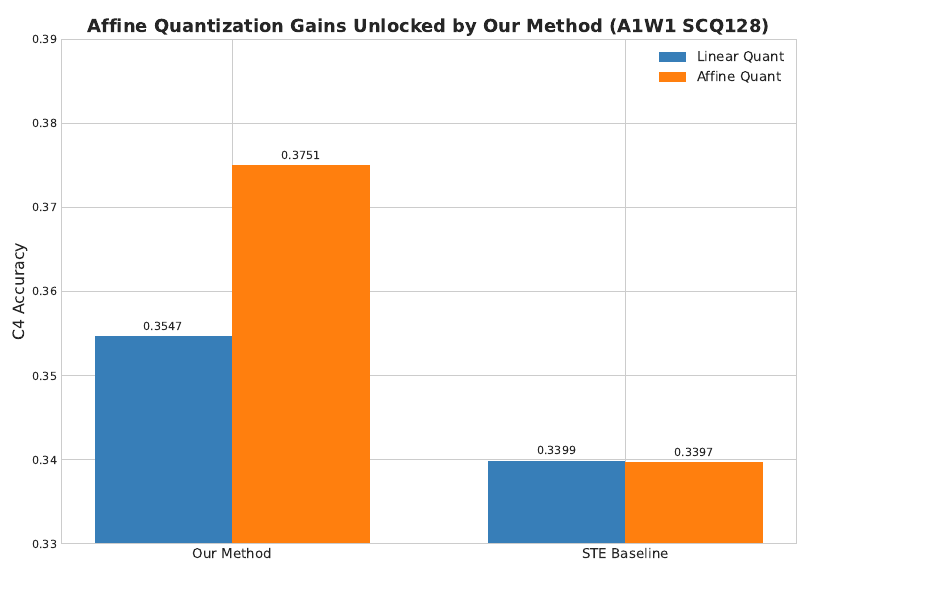
\includegraphics[height=55mm]{figs/fig1b_affine.png}
\end{center}

\paragraph{Setup.} A1W1 (1-bit weights and activations), SCQ128 (one block = 128 weights), metric = next-token accuracy on C4.

\paragraph{What the figure shows.}
\begin{itemize}
\item STE: linear $0.3399$, affine $0.3397$. Affine gives nothing.
\item Ridge: linear $0.3547$, affine $0.3751$. Affine gives $+0.020$.
\item Even ridge-linear beats STE-affine.
\end{itemize}

\paragraph{Why at 1 bit.} One bit means two levels. Linear gives two levels symmetric about zero, $\{-s,+s\}$: one free number. Affine gives two levels $\{b,\,b+s\}$: two free numbers, so both levels can sit where the weights actually are. Affine is strictly more expressive; the question is whether the method uses it.

\paragraph{STE does not use it.} The levels are $s_f$, $b_f$, fixed by $x_{\min}$, $x_{\max}$ before rounding. At 1 bit every weight is reconstructed as either $x_{\min}$ or $x_{\max}$, the two most extreme values, and the gradient carries no information about how well the levels fit ($\delta$ is invisible). The extra offset is set by the extremes, not by the data.

\paragraph{Ridge does.} $g(q)=s_g q+b_g\mathbf 1$ is a least-squares fit of $x$ on $q$. With $q\in\{0,1\}$ (and $\lambda\to0$) the fitted levels are
\[
g(0)=\text{mean of the weights rounded to }0,\qquad g(1)=\text{mean of the weights rounded to }1,
\]
the two cluster means: the best possible two levels for the current assignment. Linear ridge has only $s_g$, so its levels are forced to be symmetric; affine ridge places each level independently. And because $s_g$, $b_g$ depend on $q$, the gradient tells earlier layers how the assignment affects the fit.

\paragraph{One line.} Affine adds a free offset; only a dequantizer that is fitted to the data (ridge) can put that offset to use.

\paragraph We have two kinds of quantization: linear, which is just scaling, and affine, which is scaling plus shifting. Because of the shift, affine has more flexibility. At 1 bit this matters most, since each block gets only two levels. STE wastes that flexibility: it sets $s_f$ and $b_f$ from the smallest and largest weight in the block, so if one weight is an outlier, one of the two levels is spent on it and everything else is squashed onto the other. And STE's gradient cannot see this, so training never fixes it. Ridge instead fits the two levels to the weights, so each level sits at the average of its group, and its gradient knows how good that fit is. That is how, at 1 bit, ridge unlocks the flexibility affine provides.

\section{Short notes on the fix (slides 6--8)}

\paragraph{$N$.} The number of values in one block (the group sharing one $s_g,b_g$). Ours: one row. Paper (SCQ128): $N=128$. The $\frac1N$ turns the squared-error sum into an average.

\paragraph{$\mathrm{Var}(q)$ and $\mathrm{Cov}(x,q)$.} Within one block,
\[
\mathrm{Var}(q)=\frac1N\sum_i(q_i-\bar q)^2,\qquad \mathrm{Cov}(x,q)=\frac1N\sum_i(x_i-\bar x)(q_i-\bar q).
\]
At 1 bit: $q=(1,1,0,0)$ gives $0.25$ (the maximum); all codes equal gives $0$.

\paragraph{$\lambda$ as ridge regression.} Target $x$, feature $q$, weight $s_g$, intercept $b_g$ (not penalised). $\frac\lambda2 s_g^2$ is the usual L2 penalty:
\[
s_g=\frac{\mathrm{Cov}}{\mathrm{Var}+\lambda}=s_{\text{OLS}}\cdot\frac{\mathrm{Var}}{\mathrm{Var}+\lambda}.
\]
It shrinks $s_g$ slightly toward 0, stops it blowing up when $\mathrm{Var}(q)\approx0$, and trades a little bias for less variance. It also lowers $\rho=s_g/s_f$. With $\lambda=0.01$ it only matters in near-degenerate blocks.
\emph{To say:} ``$\lambda$ is a standard ridge penalty on the scale $s_g$; it shrinks it slightly and keeps it from blowing up when the codes have almost no spread.''

\paragraph{Why ``denoising''.} Rounding is treated as noise: $q$ is a noisy copy of $x$. STE plays the noisy copy back as is (levels at min/max). $g$ fits the best line, so each level sits near the mean of the weights it stands for. $\lambda$ sets how hard the fit is smoothed. The paper calls it a ``denoising'' knob (Sec.~3.3, App.~on $\lambda$): as $\lambda\to\infty$, $s_g\to0$ and $g$ collapses to the mean $\bar x$, ignoring the noisy $q$. Without it, a zero-variance block divides by zero and training diverges (their Table~13, $\lambda=0$). $\lambda=10^{-4}$ is fine at $\ge4$ bits; 0.01 is the safe default for 1 bit.

\paragraph{``Half pruned'' (slide 8).} Half the weights are set to exactly 0. The pattern is 2:4: in every 4 consecutive weights, keep the 2 largest in magnitude and zero the other 2. Zeros need no storage and no multiply; hardware supports 2:4. Pruning is treated as more rounding error ($x\to x_S\to q\to g(q)$), with linear quantization so 0 stays 0. Result: Gemma 3 4B, 1-bit weights, 2:4 sparse, 650\,MB, score 0.452, vs.\ 1B full precision, 1400\,MB, 0.449.

\section{The gradient with $g$ (slide 7)}

\paragraph{STE is still used.} Ridge keeps $q=f(x)+\mathrm{stopgrad}(\delta)$, so $\partial q/\partial x=I/s_f$ in both methods. $f$ is the same in both; only the rebuild after $q$ changes ($\hat x\to g$).

\paragraph{Local times upstream.} $\nabla_xL=(\text{local})^\top\,\nabla_gL$. The upstream gradient $\nabla_gL$ comes from the rest of the network.
STE: local $=\frac1{s_f}\frac{\partial\hat x}{\partial q}=I$, so $\nabla_xL=\nabla_{\hat x}L$, the same for every $\delta$.

\paragraph{Two paths with $g$.} $x$ reaches $g$ through $q$ ($x\to q\to g$) and directly through the fit ($x\to s_g,b_g\to g$):
\[
\nabla_xL=\Big(\underbrace{\tfrac1{s_f}\tfrac{\partial g}{\partial q}}_{\text{through }q}+\underbrace{\tfrac{\partial g}{\partial x}}_{\text{through }x}\Big)^{\!\top}\nabla_gL.
\]
$s_g,b_g$ also depend on $q$; that dependence sits in path 1 and is where $\delta$ enters.

\paragraph{Path 2: $\partial g/\partial x$ ($q$ fixed).} Let $u=q-\bar q\mathbf 1$, $D=N(\mathrm{Var}_q+\lambda)$. Since $\sum u_i=0$, $\mathrm{Cov}(x,q)=\frac1N\sum x_iu_i$, so
\[
\frac{\partial s_g}{\partial x}=\frac uD,\qquad \frac{\partial b_g}{\partial x}=\frac{\mathbf 1}N-\bar q\,\frac uD,
\]
\[
\frac{\partial g}{\partial x}=q\Big(\frac{\partial s_g}{\partial x}\Big)^{\!\top}+\mathbf 1\Big(\frac{\partial b_g}{\partial x}\Big)^{\!\top}=\frac{\mathbf 1\mathbf 1^\top}N+\frac{uu^\top}{D}=P.
\]
$P$ is the regression hat matrix: with $q$ fixed, $g=Px$ is linear in $x$. $\frac{\mathbf 1\mathbf 1^\top}N$ shifts the mean; $\frac{uu^\top}D$ tilts the slope. It is built from $q$ only: no $r$, no $\delta$. Hence ``no information about the rounding error''.

\paragraph{Path 1: $\partial g/\partial q$.} With $r=x-g$ and the identity $x-\bar x\mathbf 1=r+s_gu$:
\[
\frac{\partial s_g}{\partial q}=\frac{r-s_gu}{D},\qquad \frac1{s_f}\frac{\partial g}{\partial q}=\rho(I-P)+c\,u\,r^\top,\quad \rho=\frac{s_g}{s_f},\ c=\frac1{s_fD}.
\]
The residual $r$ carries $\delta$ into the gradient.

\paragraph{Total.} $J_g=P+\rho(I-P)+c\,u\,r^\top$ vs.\ $J_{\text{STE}}=I$. At high bits $\rho\to1$, $r\to0$, so $J_g\to I$ (STE); at 1 bit the error term matters most.

\end{document}
